\chapter{Électronique des improved Resistive Plate Chamber}
\label{time}
\renewcommand\chapterillustration{ELE/ele}
\ThisULCornerWallPaper{1}{\chapterillustration}
\minitoc

\lettrine[lines=4, slope=-0.5em]{C}{e} chapitre présente le développement d'un nouveau type de PCB avec lecture des deux côtés des \textit{strips}. Cette configuration permet, grâce au temps de propagation du signal de connaître la position du \textit{hit} le long du \textit{strip} touché. Ce chapitre présente également les premiers résultats obtenus lors de tests en faisceaux au SPS en mai 2017.
\vspace{-0.3cm}
\section{Principe de fonctionnement}
\vspace{-0.5cm}
Chaque chambre actuelle de CMS a un PCB segmenté en trois zones selon $\eta$ appelées "$\eta$ segments", chaque $\eta$ segment contenant \num{32} \textit{strips}. Lors du passage d'un muon, la position de celui-ci selon $\eta$ n'est connu qu'avec une résolution correspondant à la longueur du \textit{strip} touché.

Afin de résoudre ce problème et d'éviter la segmentation en $\eta$ du PCB, un type de PCB permettant la lecture des deux côtés des \textit{strips} a été proposé (cf.Fig~\ref{PCB1}).
\vspace*{-0.3cm}
\begin{figure}[ht!]
	\centering
	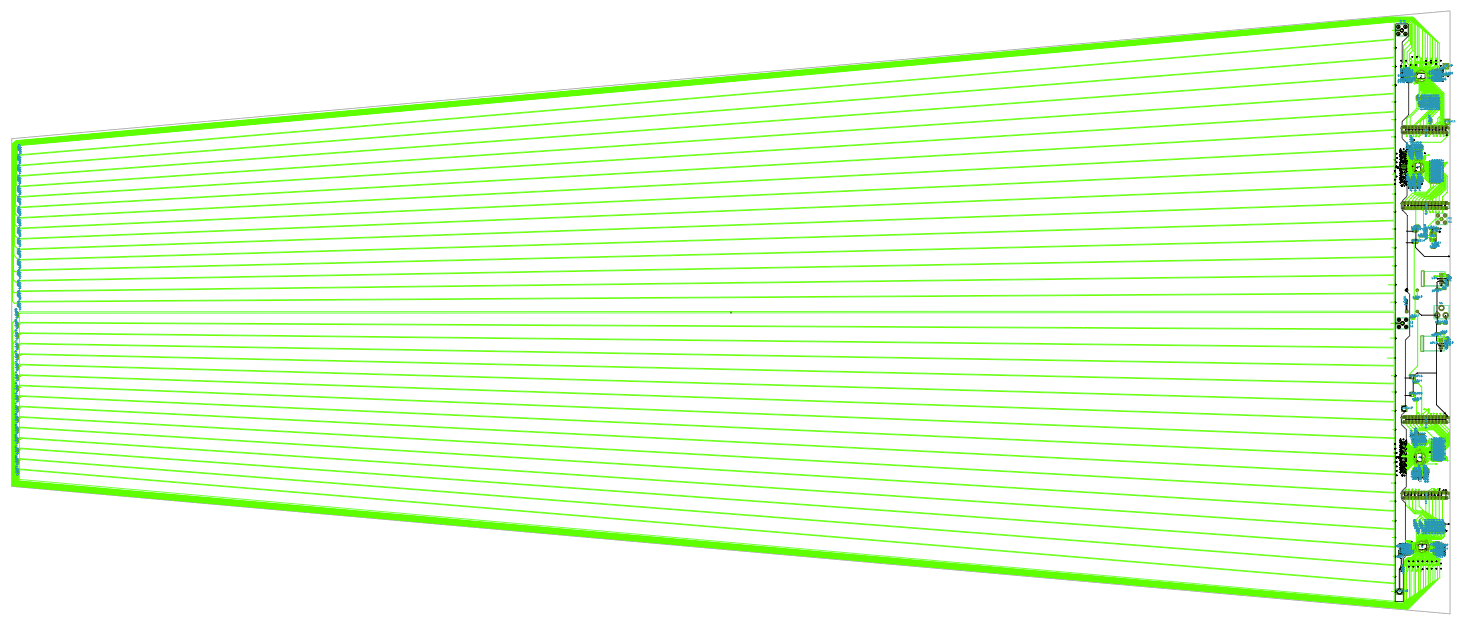
\includegraphics[width=0.50\textwidth]{ELE/PCB1.png}
	\captionsetup{type=figure}\caption{Schéma du PCB permettant la lecture des deux côtés des \textit{strips}.}
	\label{PCB1}
\end{figure}

\vspace{-0.5cm}
Les \textit{strips} font toute la longueur de la chambre, chaque extrémité des \textit{strips} est reliée à une voie d'électronique. Le retour du \textit{strip} est effectué sur les côtés du PCB, dans une zone protégée par un blindage relié à la masse afin que le retour ne soit pas affecté par le passage des particules.

Ce type de configuration permet de connaître la position d'un \textit{hit} le long du \textit{strip}. En effet en posant $Y$ la position du \textit{hit} le long du \textit{strip}, $L$ la longueur de la ligne (\textit{strip} et retour), $T_1$ et $T_2$ le temps de propagation du signal pour rejoindre l'un et l'autre côté de la ligne, $T$ le temps d'arrivée du signal sur le \textit{strip} et $v$ la vitesse de propagation du signal :
\begin{equation}
\label{eqqq}
Y=\frac{L}{2}-\frac{v(T_2-T_1)}{2}
\end{equation} 

Le temps d'arrivée du signal peut également être calculé :
\begin{equation}
\label{myformule}
T=-\frac{(T_1+T_2)}{2}+\frac{L}{2v}
\end{equation}

\section{Le Prototype}
Afin d'étudier la faisabilité, un PCB de \SI{50}{\centi\meter} de long a été créé (cf.Fig~\ref{PCB2}). Il est composé de \num{32} \textit{strip}s espacés de \SI{4}{\milli\meter}. Ces \textit{strips} sont lus de chaque côté grâce à \num{2} ASIC appelés PETIROC2 \cite{Monzo:2017quz} de \num{32} entrées chacun, développés par le groupe OMEGA. Ces ASIC sont utilisés pour mettre en forme les signaux. Deux TDC (appelés mezzanines) de \num{24} voies chacun et de résolution temporelle \SI{25}{\pico\second}, développés par nos collègues de Tsinghua sont utilisés afin de mesurer le temps d'arrivé des signaux envoyés par les PETIROC2.

\begin{figure}[ht!]
	\centering
	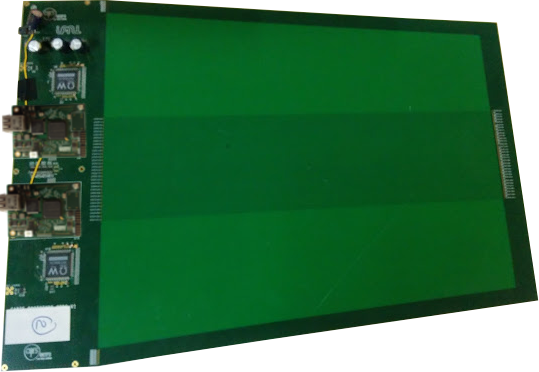
\includegraphics[width=0.77\textwidth]{ELE/PCB2.png}
	\captionsetup{type=figure}\caption{Le PCB avec lecture des \textit{strips} des deux côtés.}
	\label{PCB2}
\end{figure}

\subsection{Le TDC}
\begin{wrapfigure}[7]{R}{0.40\textwidth}
	\vspace*{-1cm}
	\centering
	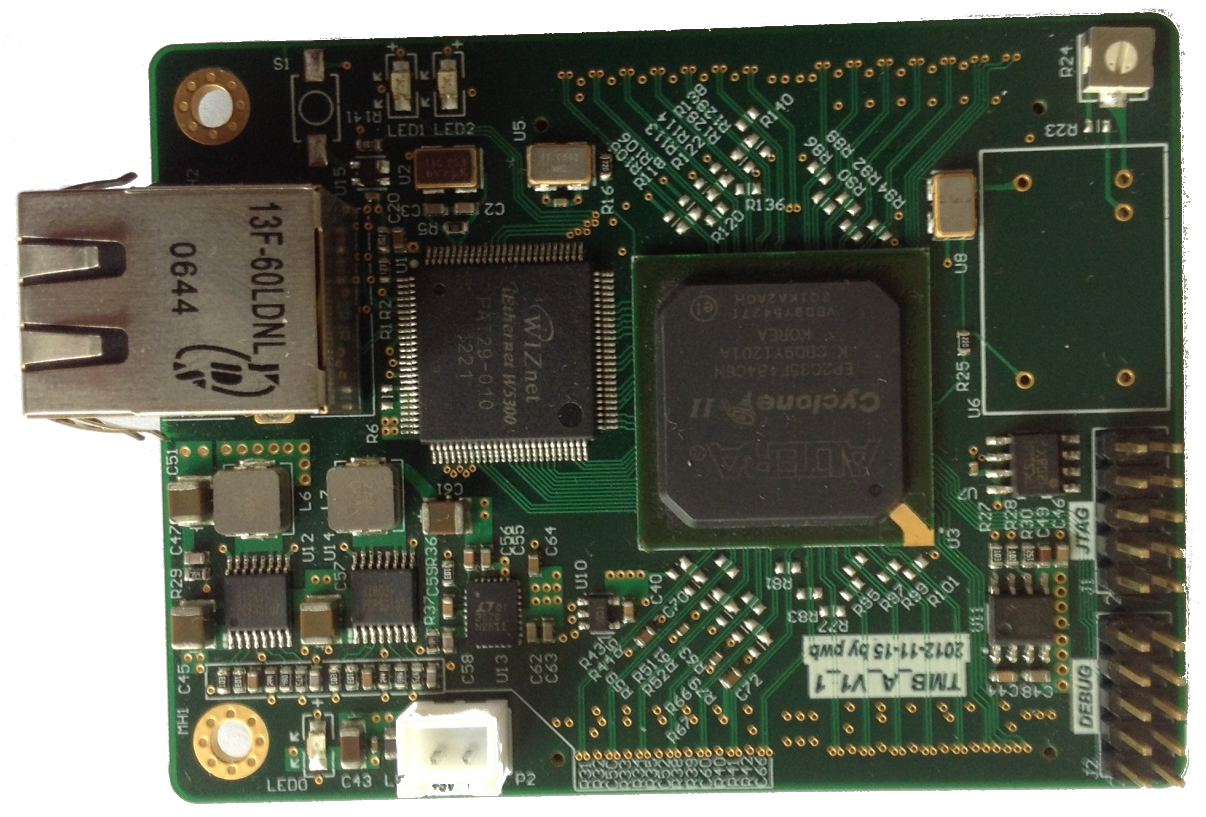
\includegraphics[width=0.30\textwidth]{ELE/TDC.png}
	\caption{Un TDC fourni par nos collègues de Tsinghua.}
	\label{tdc}
\end{wrapfigure}
Le TDC fourni par nos collègues chinois possède \num{24} voies et une résolution temporelle de \SI{25}{\pico\second}. Il est basé sur un FPGA de type Cyclone-II. Cette carte reçoit les données des PETIROC2 grâce à des connecteurs à entrées différentielles. En sortie, les données sont envoyées grâce à un port Éthernet utilisant les protocoles TCP\footnote{Transmission Control Protocol.}/IP\footnote{Internet Protocol.}.

\subsection{L'ASIC PETIROC2}

\begin{wrapfigure}[11]{R}{0.40\textwidth}
	\centering
	\vspace*{-1cm}
	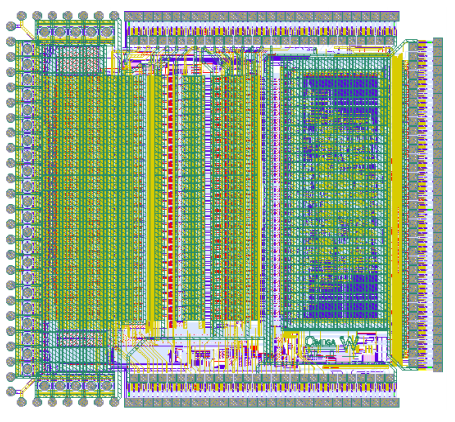
\includegraphics[width=0.25\textwidth]{ELE/PETIROC.png}
	\caption{Schéma électronique du PETIROC2.}
	\label{PETIROC2}
\end{wrapfigure}

Le PETIROC2 (cf.Fig~\ref{PETIROC2}) repose sur une technologie de fonderie AMS SiGe \SI{0.35}{\micro\meter}. La puce est insérée dans un boitier de taille \num{4.6}$\times$\SI{42}{\square\milli\meter}, d'épaisseur \SI{1.6}{\milli\meter} et comporte \num{208} pattes dont \num{32} voies d'entrée. Le schéma simplifié du PETIROC2 est donné figure \ref{SchemePETIROC}. Chaque voie permet de mesurer le temps de propagation du signal grâce à un TDC intégré et un ADC de \num{10} bits ainsi que la charge sur \num{10}bits. La gamme de réglage du seuil global aux \num{32} voies est comprise entre \SI{160}{\femto\coulomb} et \SI{400}{\pico\coulomb}. Un ajustement voie par voie est possible grâce à un DAC de \num{6} bits. 

\begin{figure}[ht!]
	\centering
	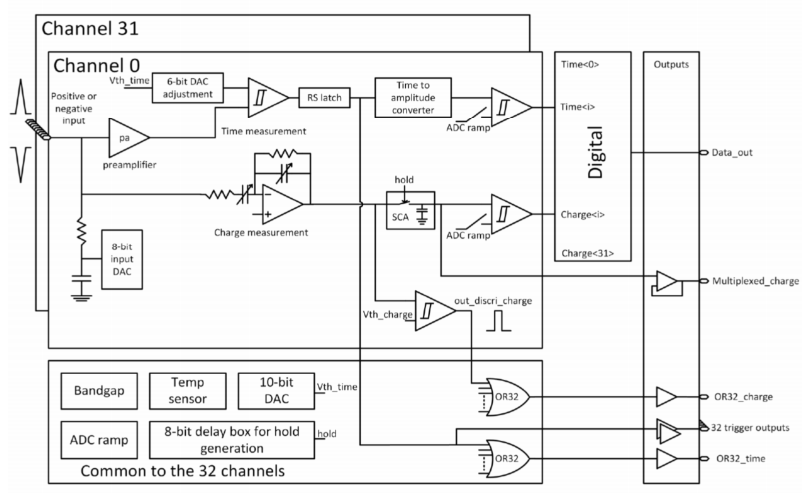
\includegraphics[width=0.65\textwidth]{ELE/Scheme.png}
	\captionsetup{type=figure}\caption{schéma simplifié du PETIROC2.}
	\label{SchemePETIROC}
\end{figure}

Le PETIROC2 possède une gigue\footnote{La gigue ou \textit{jitter} en anglais, provient des fluctuations statistiques et du bruit de l'électronique. À cause de ces fluctuations, deux signaux identiques ne vont pas passer le seuil de déclenchement au même point, donnant ainsi une variation temporelle du point de déclenchement qui dépend de l'amplitude des fluctuations.} faible ($<\SI{20}{\pico\second}$ pour une charge supérieure à \SI{1.5}{\milli\volt}) (cf.Fig~\ref{jitter}).

\begin{figure}[ht!]
	\centering
	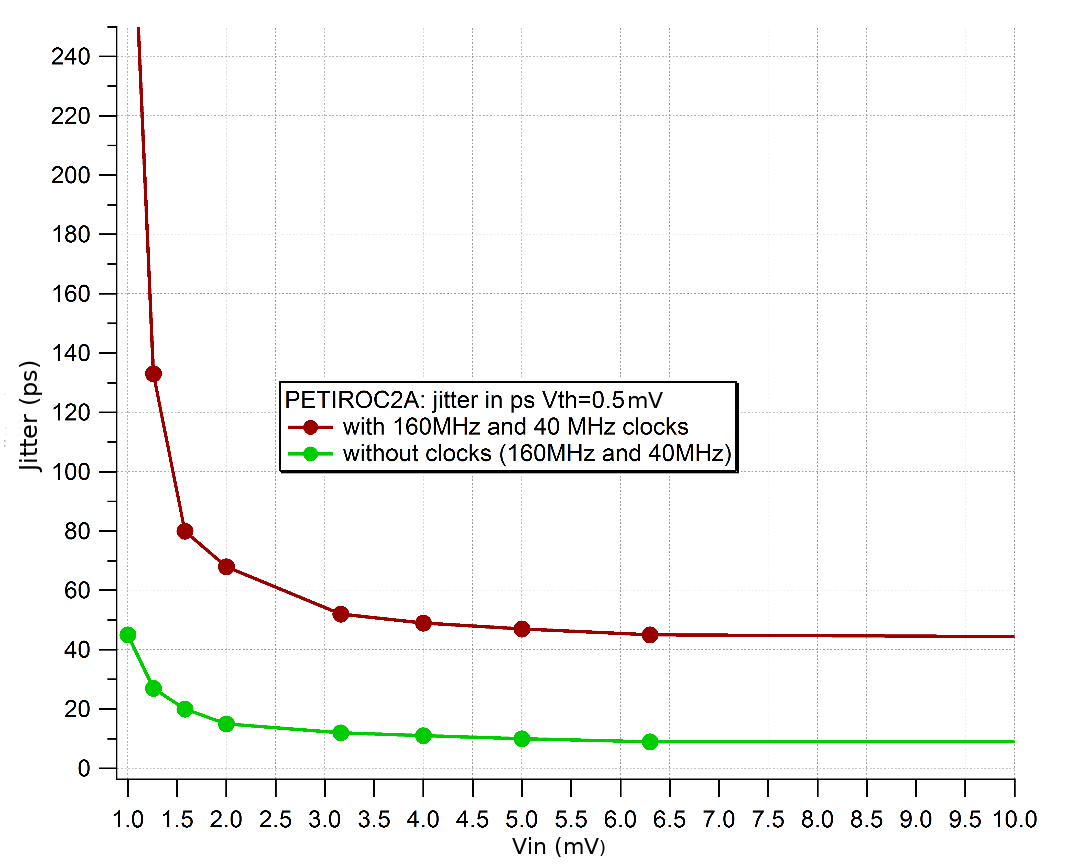
\includegraphics[width=0.65\textwidth]{ELE/Jitter.png}
	\captionsetup{type=figure}\caption{Gigue en fonction de la tension injectée. Le seuil est fixé à \SI{0.5}{\milli\volt}. Dans notre cas, la gigue est donnée par la courbe verte.}
	\label{jitter}
\end{figure}

\vspace{0.4cm}
\section{Résolution temporelle du PCB}
La résolution temporelle du PCB a été testée en injectant un signal carré de \SI{10}{\volt} d'amplitude et de durée \SI{10}{\nano\second} à travers un condensateur de \SI{1}{\pico\farad} sur des points de test (en bleu sur la figure \ref{PCB2}). Un exemple de la distribution temporelle de $T_{1}-T_{2}$ pour un \textit{strip} est donné figure \ref{RESOLUTION}

\begin{figure}[!ht]
	\centering
	\scalebox{1.5}{\includetex{ELE/TDCTimeResolution}}
	\caption{Résolution temporelle d'un \textit{strip} du PCB. Le signal est un carré d'amplitude \SI{10}{\volt} et de durée \SI{10}{\nano\second}. Le signal traverse un condensateur de \SI{1}{\pico\farad}.}
	\label{RESOLUTION}
\end{figure}

Un ajustement de la distribution temporelle de $T_{1}-T_{2}$ par une Gaussienne est effectué. La valeur moyenne de la Gaussienne n'est pas pertinente car les TDC n'ont pas été calibrés. Cependant, l'écart type $\sigma$ de la Gaussienne permet de déduire la résolution temporelle du PCB. En effet, en supposant les variables $T_1$ et $T_2$ décorrélées on a
\begin{equation}
\sigma_{T_1+T_2}=\sqrt{\sigma_{T_1}^2+\sigma_{T_2}^2}.
\end{equation}
En supposant de plus que $\sigma_{T_1}^2=\sigma_{T_2}^2=\sigma_{elec}^2$
\begin{equation}
\frac{\sigma_{T_1+T_2}}{\sqrt{2}}=\sigma_{elec}.
\end{equation}
La résolution temporelle du PCB est estimée entre \SI{20}{\pico\second} et \SI{30}{\pico\second}.

\section{Test en faisceaux au SPS (mai 2017)}
\label{TIMINGG}
\vspace{-0.4cm}
Deux chambres double \textit{gaps} en Bakélite de \textit{gap} \SI{1.4}{\milli\meter} (\SI{1.6}{\milli\meter}) et épaisseur d'électrodes \SI{1.4}{\milli\meter} (\SI{1.6}{\milli\meter})\footnote{Ce sont les deux types de chambres privilégiées par le TDR.} ont été instrumentées avec le PCB à \textit{strips} et testées sur la ligne H4 du SPS dans la \textit{North Area} (cf.Fig~\ref{complexe}). Les chambres ont été posées sur une table de positionnement réglable verticalement et horizontalement (cf.Fig\ref{setup2017}).
\begin{figure}[ht!]
	\centering
	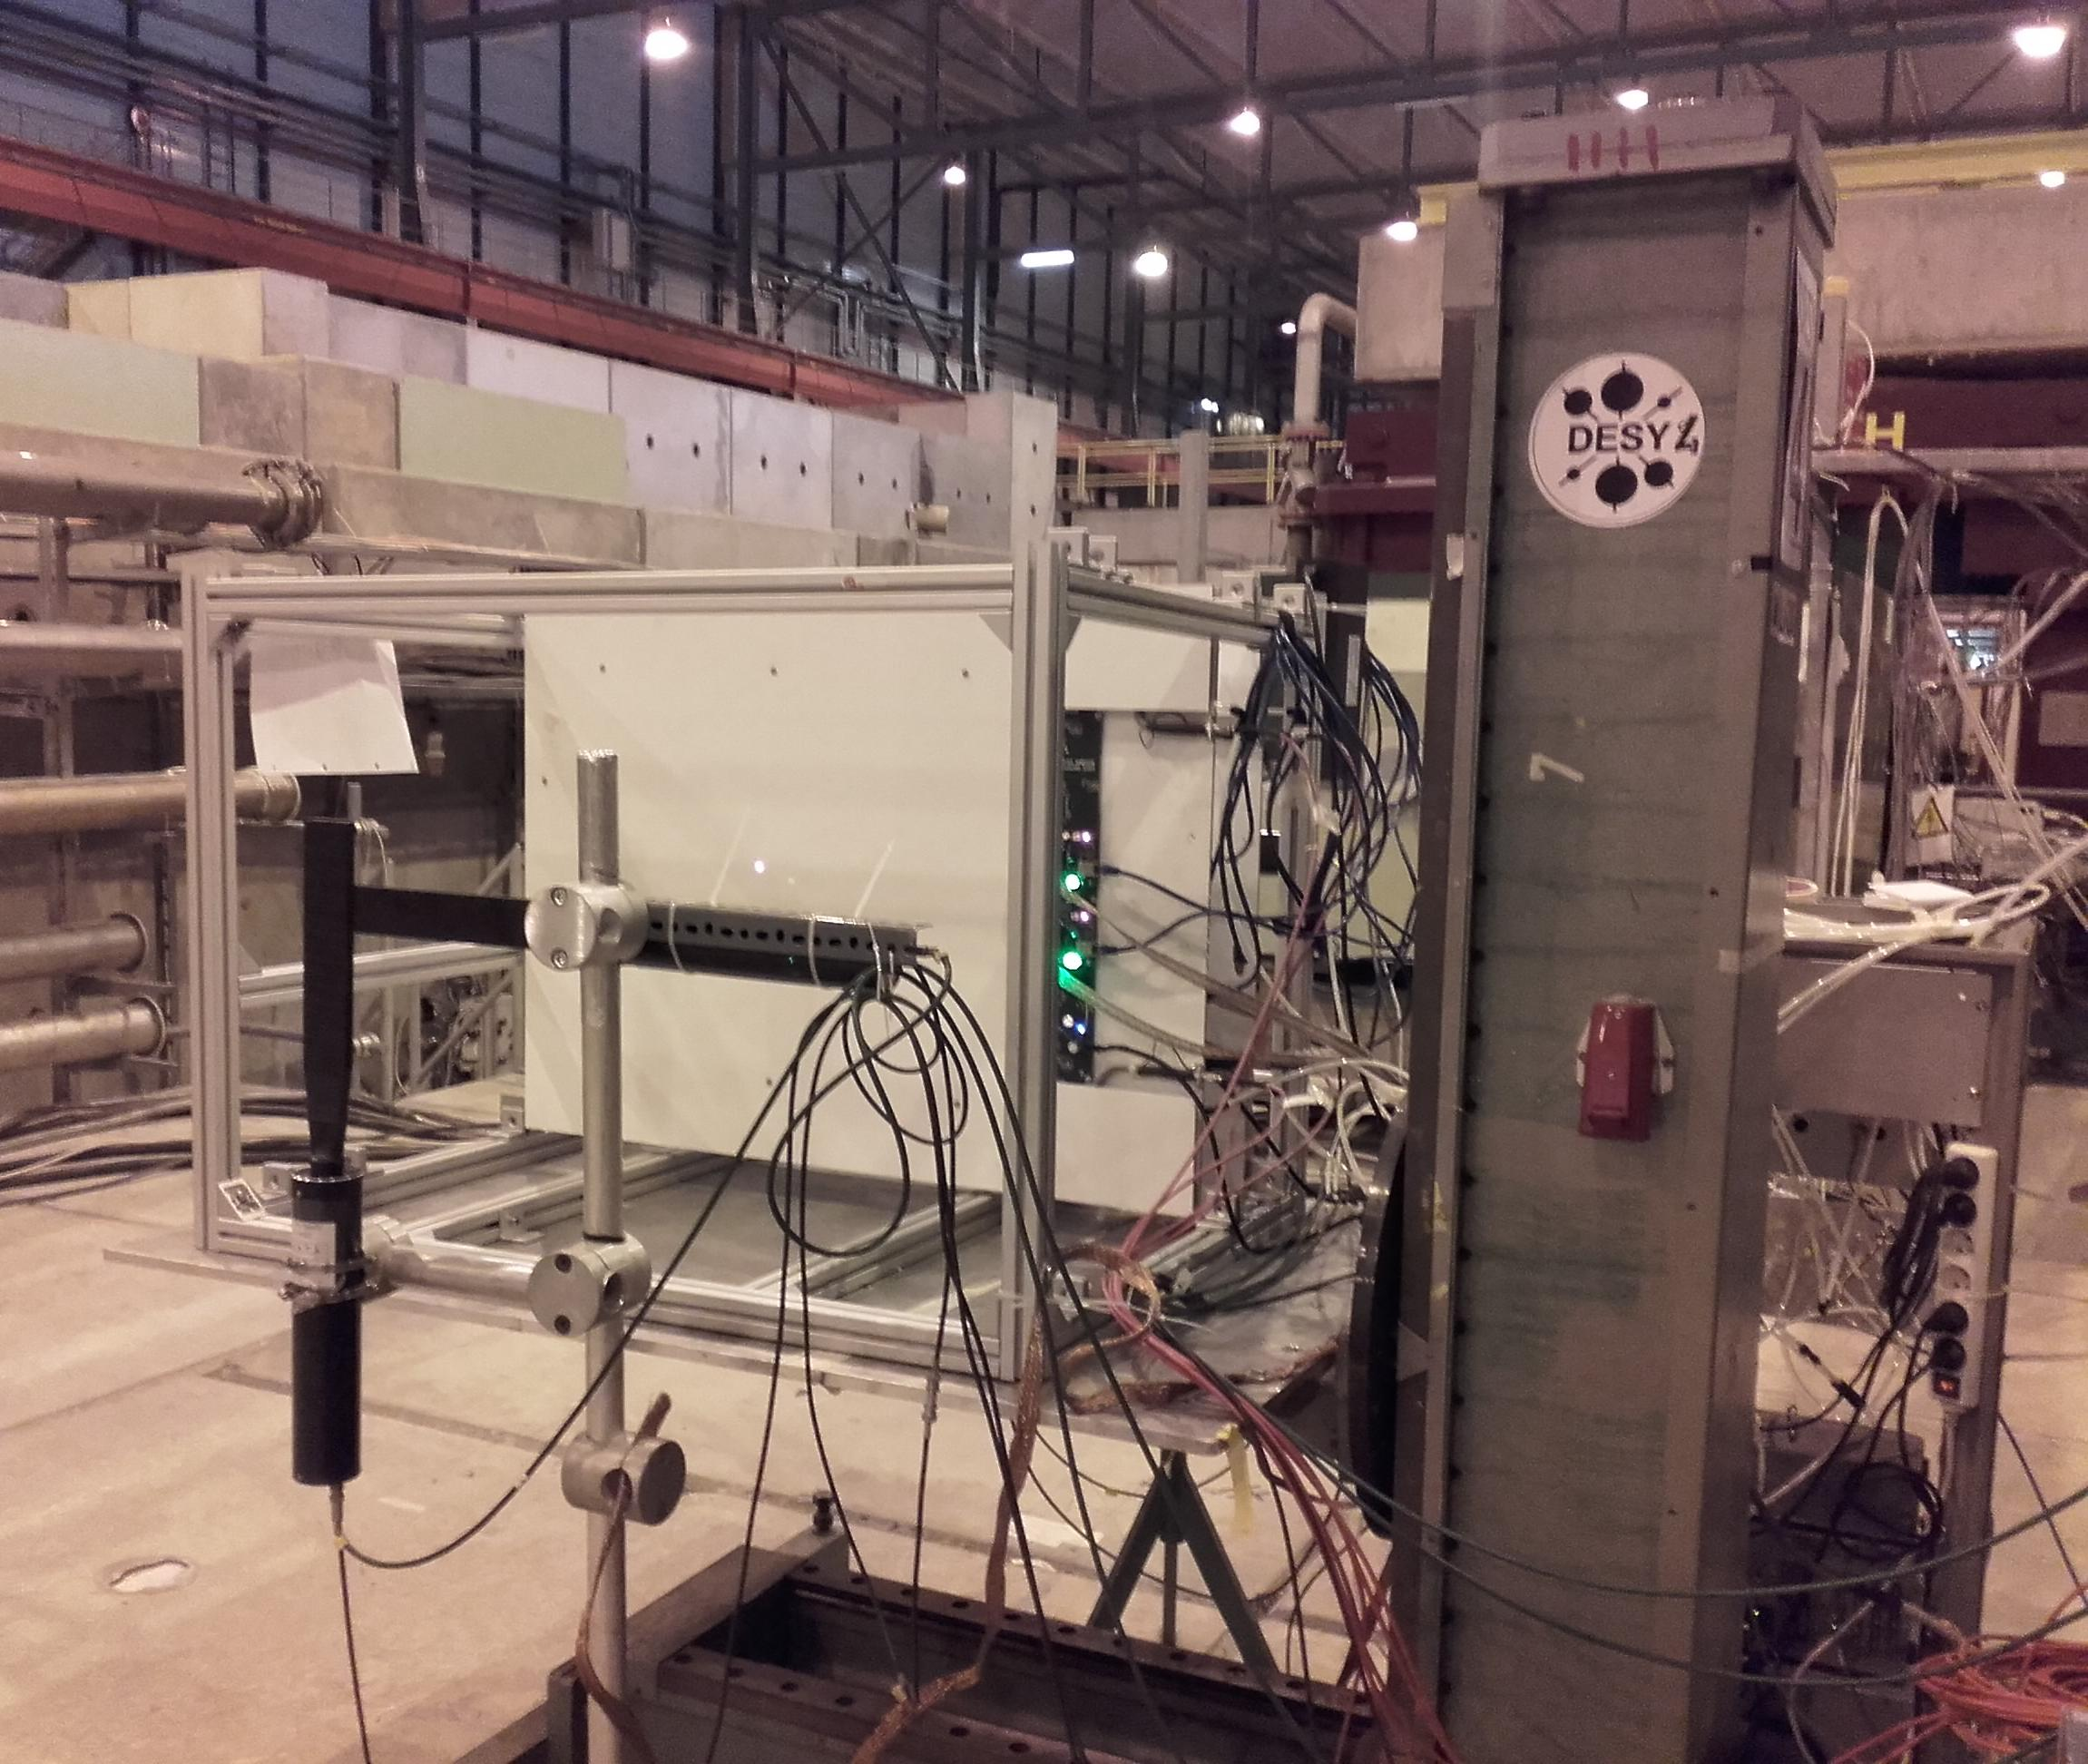
\includegraphics[width=0.55\textwidth]{ELE/setup2017.jpg}
	\captionsetup{type=figure}\caption{Les deux chambres en Bakélite posées sur la table de positionnement.}
	\label{setup2017}
\end{figure}

Deux groupes de deux PM de \SI{5}{\centi\meter} de largeur sont placés de part et d'autre des chambres. Les PM d'un même groupe sont placés perpendiculairement l'un par rapport à l'autre (cf.Fig~\ref{setup2017}). 

Deux autres PM de plus petites dimensions (\SI{1.2}{\centi\meter}) sont placés d'un côté des chambres afin de réduire la zone de déclenchement (cf.Fig~\ref{smallPM}).  

\marginpar
{
	\centering
	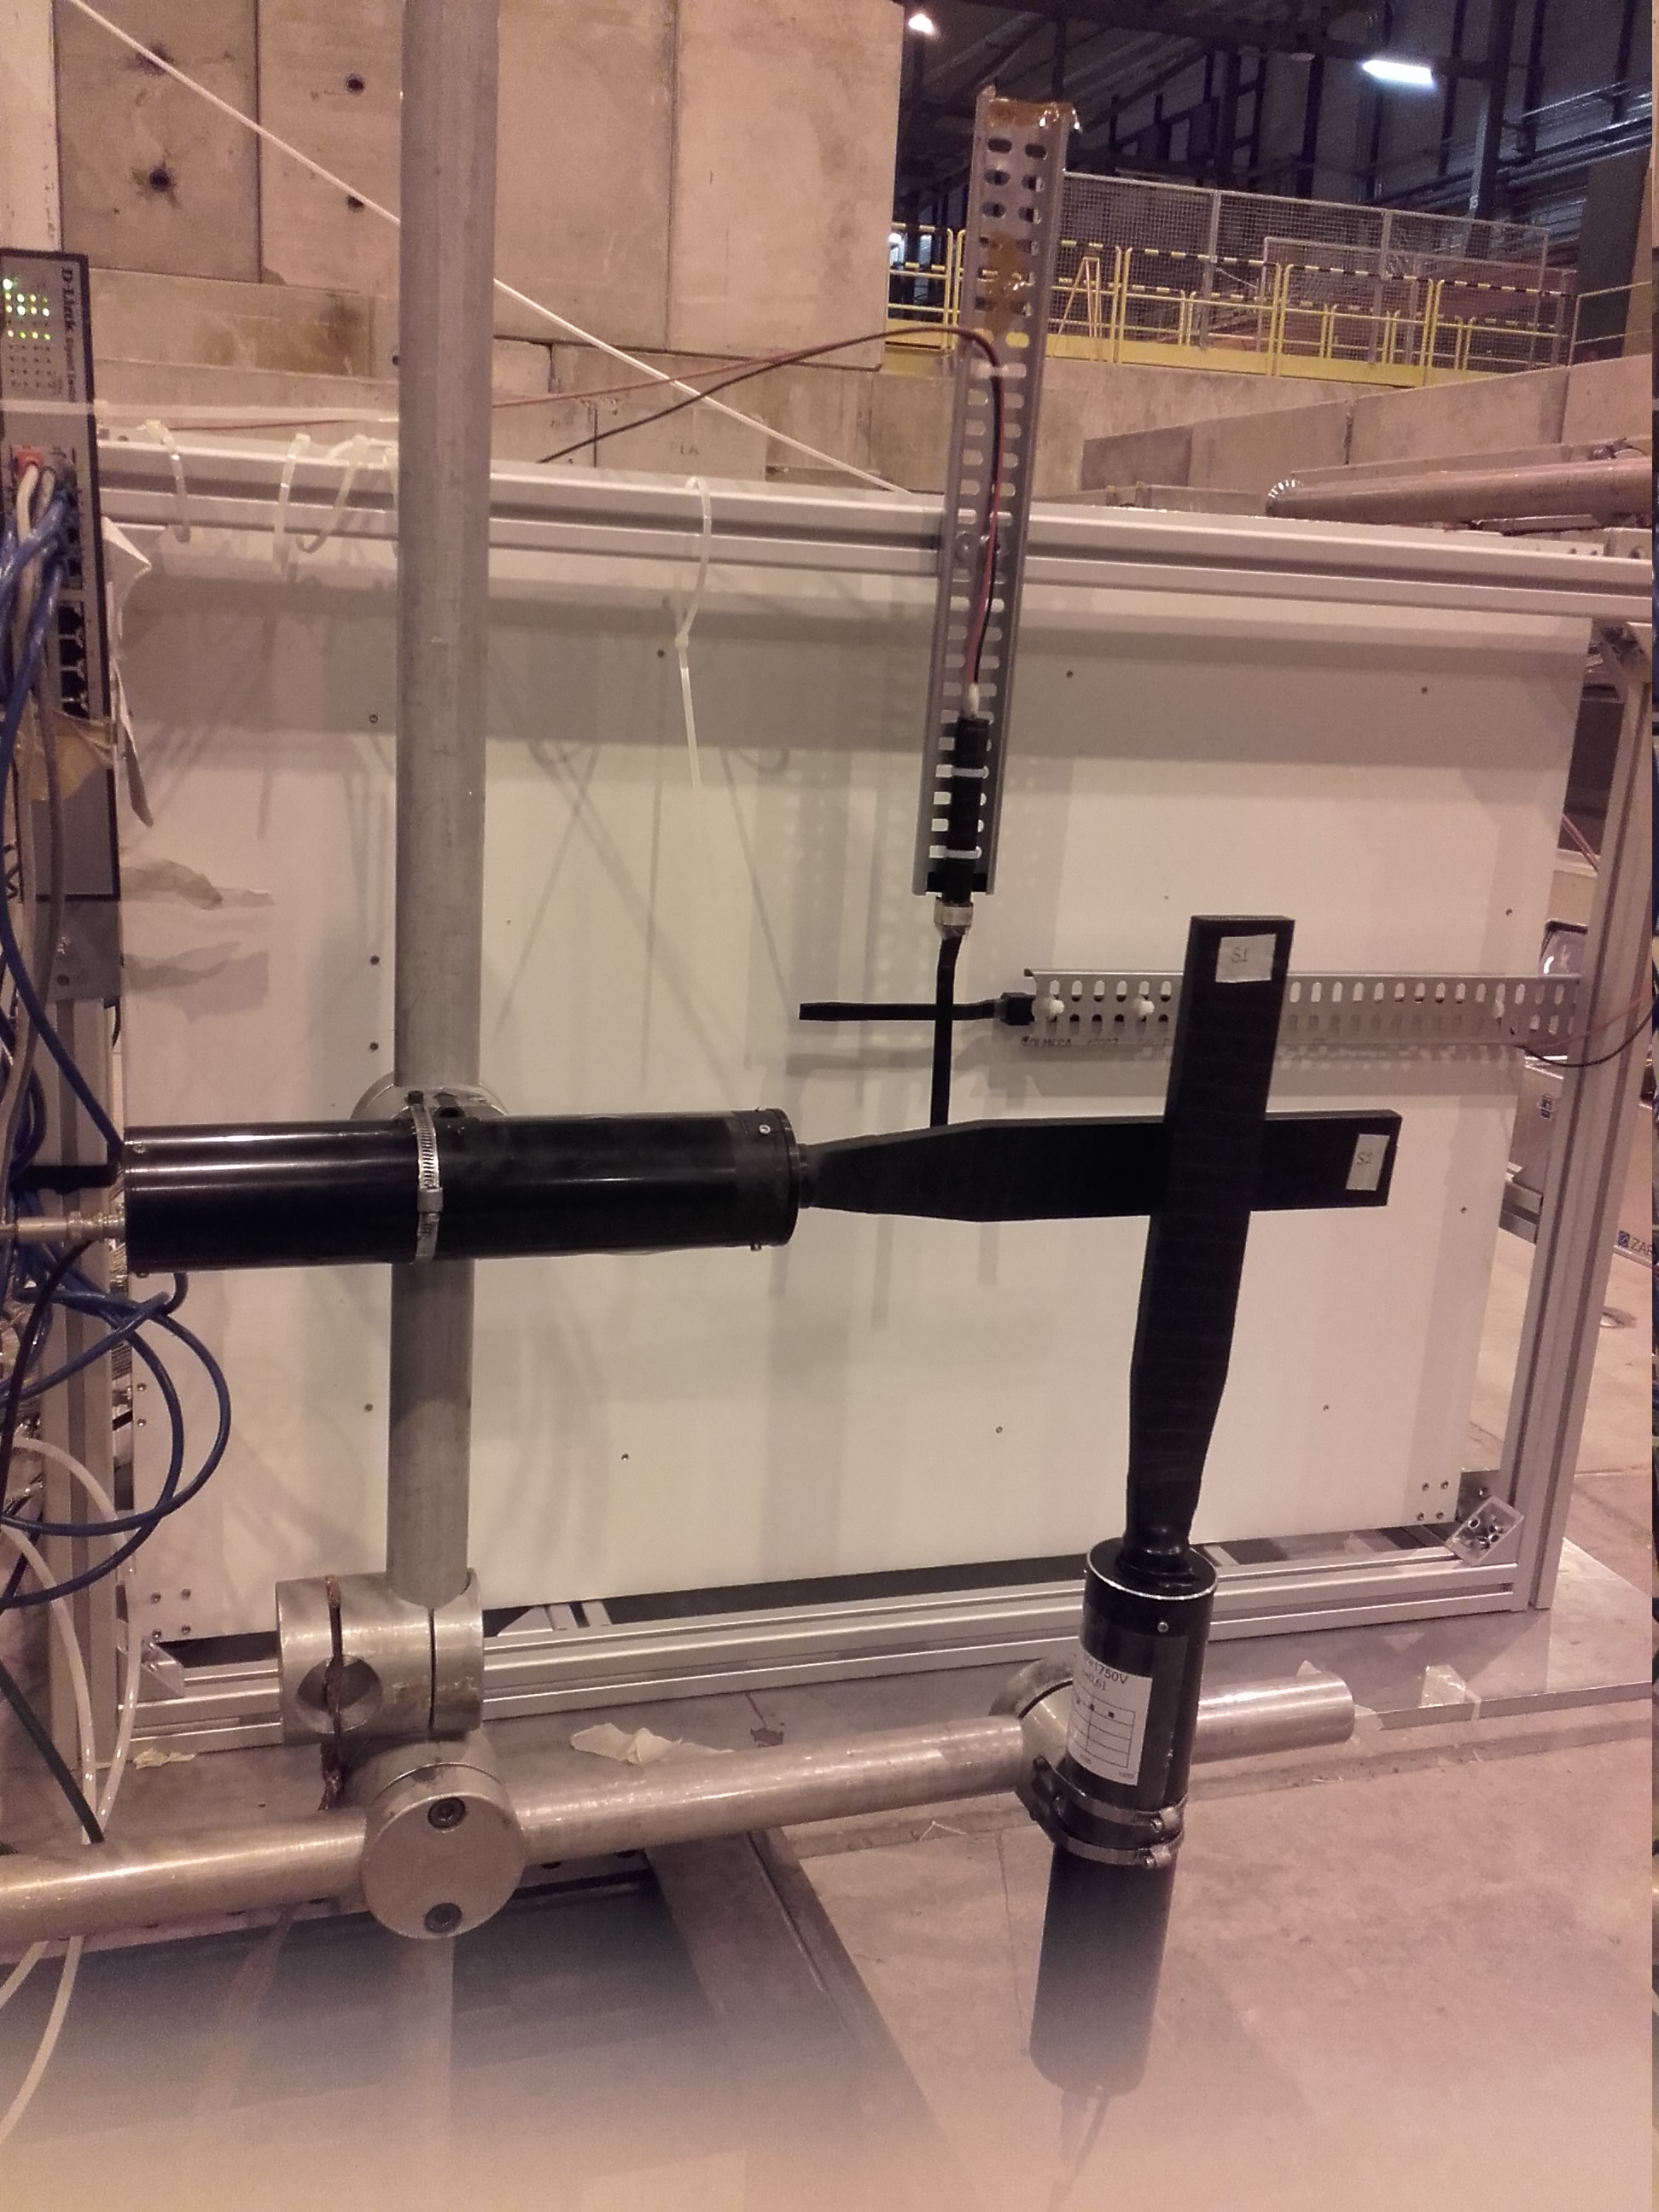
\includegraphics[width=\marginparwidth]{ELE/BigSmallScintillators.jpg}
	\captionsetup{type=figure}\caption{Les différents PM placés d'un côté des chambres.}
	\label{smallPM}
}

La coïncidence des scintillateurs est envoyée dans les données comme s'il s'agissait du signal d'un \textit{strip}. Chaque mezzanine reçoit le signal de coïncidence.
\vspace*{-0.4cm}
\subsection{Format de données}
\vspace*{-0.4cm}
Les événements sont envoyés par TCP/IP et enregistrés sous forme de blocs binaires. Les informations codées dans ces blocs sont données tableau \ref{donnees}. Chaque Mézzanine est identifiable par son adresse IP, le côté des \textit{strips} dont elle s'occupe est identifiable par "Numéro mezzanine" (\num{0} ou \num{1}). Pour chaque \textit{strip} touché est enregistré le numéro de la voie du PETIROC2 correspondant, le temps permettant de se repérer dans un événement (BCID) de résolution \SI{200}{\nano\second} et le temps enregistré par le TDC (Coarse et Fine).

\begin{table}[!ht]
	\centering
\begin{tabular}{|OOO|O|N}
	\hline
	\multicolumn{3}{|c|}{Contenu d'un événement}& Taille (octets) \\ 
	\hline
	\multicolumn{3}{|c|}{Nombre de mezzanine $N_{mez}$}& 4 \\ 
	\hline
	\multirow{13}{1.5cm}{$N_{mez}\times $}&\multicolumn{2}{|c|}{Detector Id}& 4 \\ \cline{2-4}
	&\multicolumn{2}{|c|}{Datasource Id }& 4 \\ \cline{2-4}
	&\multicolumn{2}{|c|}{Event Id }& 4 \\ \cline{2-4}
	&\multicolumn{2}{|c|}{Bunch Crossing Id}& 8 \\ \cline{2-4}
	&\multicolumn{2}{|c|}{Numéro d'évènement}& 4 \\ \cline{2-4}
	&\multicolumn{2}{|c|}{Global Trigger Counter (GTC)}&4\\\cline{2-4}
	&\multicolumn{2}{|c|}{BCID mezzanine}&8\\\cline{2-4}
	&\multicolumn{2}{|c|}{Numéro mezzanine}&4\\\cline{2-4}
	&\multicolumn{2}{|c|}{IP Mézzanine}&4\\\cline{2-4}
	&\multicolumn{2}{|c|}{Nombre de voies touchés $N_{touch}$}&4\\\cline{2-4}
	&\multicolumn{1}{|c|}{\multirow{3}{1.5cm}{$N_{touch}\times $}}&Numéro de la voie&1\\\cline{3-4}
	&\multicolumn{1}{|c|}{}&BCID Strip&2\\\cline{3-4}
	&\multicolumn{1}{|c|}{}&Coarse&4\\\cline{3-4}
	&\multicolumn{1}{|c|}{}&Fine&1\\\cline{3-4}
	\hline
	\multicolumn{3}{|c|}{Total}&$4+N_{mez}\times(48+N_{touch}\times8)$\\
	\hline
\end{tabular}
\caption{Contenu d'un événement et sa taille en octets.}\label{donnees}
\end{table}

\newpage
Le démarrage et l'arrêt de l'acquisition sont pilotés grâce à un générateur de fonctions qui envoie un créneau. Un événement tel que décrit dans la table \ref{donnees} est envoyé pour chaque créneau. Un signal \textit{"busy"} est activé afin de bloquer la prise de données pendant l'exportation des données vers l'ordinateur.

\subsection{Programme d'analyse}
Le programme d'analyse est écrit en \Cpp en utilisant ROOT. Il permet de lire les données binaires et de chercher les \textit{hits} correspondant à la coïncidence des scintillateurs et de déterminer leur temps TDC $T_0$. Afin de simplifier l'analyse, seuls les événements comportant un seul \textit{hit} de ce type sont sélectionnés. Les événements comportant un nombre de \textit{hits} trop important ($>1000$) sont également rejetés.

Pour chaque \textit{hit} de l'événement, le temps d'arrivé $T$ de celui-ci par rapport au signal des scintillateurs est calculé :
\begin{equation}
	T^n=T'^n-T_0
\end{equation}
avec $T'$ la valeur du temps TDC du \textit{hit} $n$. 

Un ajustement par une fonction Gaussienne de la distribution des $T^n$ est ensuite effectué. La distribution présentant de nombreux pics (cf.Fig~\ref{pics}), seule la zone proche du premier pic (proche du temps $T_0$) est prise en compte dans l'ajustement. La zone correspondant au signal est ensuite prise comme étant l'intervalle $\left[T_0-\num{1.5}\sigma,T_0+\num{1.5}\sigma\right]$.

\begin{figure}[!ht]
	\centering
	\scalebox{0.45}{\includetex{ELE/Pic}}
	\caption{Distribution des $T^n$ pour une chambre et ajustement par une fonction Gaussienne de la zone proche du premier pic.}
	\label{pics}
\end{figure}

Pour chaque \textit{strip}, la distribution des $T^{n,s}_1-T^{n,s}_2$ où $T^{n,s}_1=T_{n,s}^{'1}-T_0$ est le temps du \textit{hit} $n$ du \textit{strip} $s$ par rapport au temps du signal des scintillateurs $T^{0}$ lu d'un côté et $T^{n,s}_2$ celui lu par l'autre côté du \textit{strip}.

La figure \ref{t2t0} représente la distribution des $T^{n,21}_2$ de la chambre en Bakélite \SI{1.4}{\milli\meter}.
\begin{figure}[ht!]
	\centering
	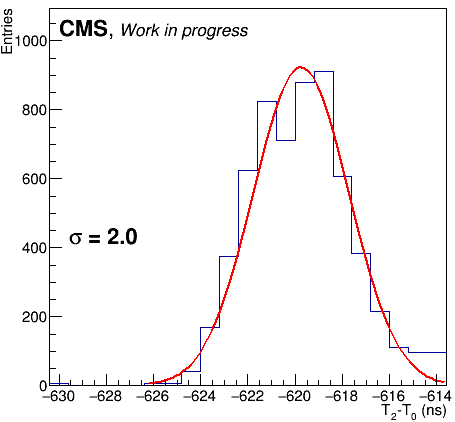
\includegraphics[width=0.40\textwidth]{ELE/TimingFitsRunT1T0_zoom_736185.jpg}
	\captionsetup{type=figure}\caption{Distribution des $T^{n,21}_2$ de la chambre en Bakélite \SI{1.4}{\milli\meter}.}
	\label{t2t0}
\end{figure}

La figure \ref{t2t0} permet d'en déduire que :
\begin{equation}
\sigma_{T_2-T_0}=\sqrt{\sigma_{T_2}^2+\sigma_{T_0}^2}=\SI{2.0}{\nano\second}
\end{equation}

Malheureusement nous ne connaissons pas $\sigma_{T_0}^2$ afin d'en déduire $\sigma_{T_2}^2$. De plus les TDC n'ont pas été calibrés avant le test en faisceaux, ce qui affecte les résolutions.

Le programme effectue le calcul de l'efficacité des chambres ainsi  qu'une clusterisation d'un côté et de l'autre afin d'obtenir le \textit{cluster size} et la probabilité de \textit{streamer}. Cependant, le signal reçu par les \textit{strips} est très atténué du fait de l'importante épaisseur (\SI{1.5}{\milli\meter}) du PCB en plus du Mylar.% Cependant, le PCB s'est avéré très épais \SI{750}{\micro\meter} de chaque côté des \textit{strips}, en plus du Mylar, ce qui atténue le signal reçu par les \textit{strips}.

\subsection{Résultats}


\subsubsection{Courants}
Avant de nous intéresser aux précisions spatiale et temporelle obtenues par ces chambres nous avons effectué des balayages en tension afin d'obtenir leurs courbes d'efficacités et de courants. Ces chambres étant nouvelles et n'ayant jamais été testées, nous voulions nous assurer de leur bon fonctionnement.

La différence de courants parcourant les chambres entre les périodes sans faisceaux et avec faisceaux en fonction de la haute tension appliquée est donnée par la figure \ref{courant1.4} (\ref{courant1.6}) pour la chambre \SI{1.4}{\milli\meter} (\SI{1.6}{\milli\meter}).

\begin{figure}[ht!]
	\vspace{-0.5cm}
	\centering
	\subfloat[chambre \SI{1.4}{\milli\meter}.]{\scalebox{0.68}{\includetex{ELE/1p4}}\label{courant1.4}}
	\subfloat[chambre \SI{1.6}{\milli\meter}.]{\scalebox{0.68}{\includetex{ELE/1.6}}\label{courant1.6}}
	\caption{Différences de courants parcourant les chambres entre les périodes sans faisceaux et avec faisceaux en fonction de la haute tension appliquée.}
	\label{courant1.41.6}
\end{figure}

Les deux chambres ont un comportement normal. De plus leurs comportements sont identiques si l'on considère leurs différences d'épaisseur d'électrodes et de \textit{gap}.

En effet, en considérant les tensions des figures \ref{courant1.4}, \ref{courant1.6} pour lesquelles les courants augmentent linéairement et en les ajustant par une droite. Les coordonnées de ces droites nous permettent de calculer la valeur pour lesquelles elles coupent l'axe des abscisses $V^c$ (\SI{6768}{\volt} et \SI{8396}{\volt} respectivement). Les matériaux des chambres et le gaz étant identiques, on peut donc considérer qu'à ces points les champs électriques sont identiques.

\begin{equation}
E_{\num{1.4};\num{1.4}}\left( 6768 \right)=E_{\num{1.6};\num{1.6}}\left( 8396 \right)
\end{equation} 
\begin{equation}
\frac{V^c_{1.4}-2\frac{\rho L I_{1.4}}{S} }{1.4}=\frac{V^c_{1.6}-2\frac{\rho L I_{1.6}}{S} }{1.6}
\end{equation} 
où $I$ est le courant dans la chambre, $\rho$ la résistivité de la Bakélite, $L$ l'épaisseur des électrodes et $S$ la surface des chambres.

En négligeant les pertes par effet ohmique dans les électrodes et en comparant $\frac{V_{1.4}}{V_{1.6}}~=~\num{0.806}$ et $\frac{1.4}{1.6}=\num{0.875}$ on peut en déduire, qu'avec les hypothèses que nous avons avancées, les chambres ont un même comportement.

\subsubsection{Résolution spatiale}

Afin d'obtenir la résolution spatiale $\sigma_{Y}$ nous avons effectué plusieurs \textit{runs} en bougeant la table de positionnement, déplaçant ainsi la zone des \textit{strips} touchés. Les figures \ref{25p5cm}, \ref{17p5cm} et \ref{5p5cm} montre la distribution des $T^{n,21}_2-T^{n,21}_1$ pour plusieurs positions de la table. 

\begin{figure}[ht!]
	\centering
	\subfloat[Distribution des $T^{n,21}_2-T^{n,21}_1$ lorsque le faisceau est à une distance \SI{25.5}{\centi\meter} des mezzanines.]{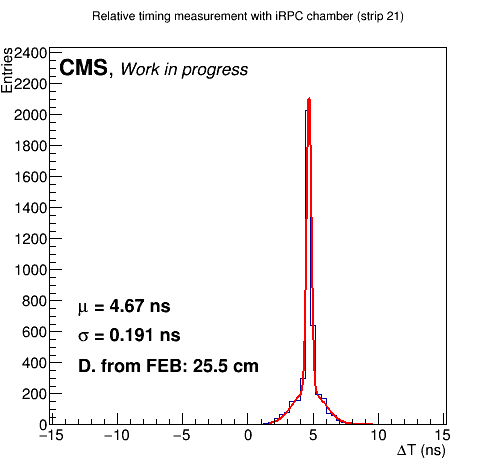
\includegraphics[width=\marginparwidth]{ELE/25p5cm.jpg}\label{25p5cm}}
	\hfill
	\subfloat[Distribution des $T^{n,21}_2-T^{n,21}_1$ lorsque le faisceau est à une distance \SI{17.5}{\centi\meter} des mezzanines.]{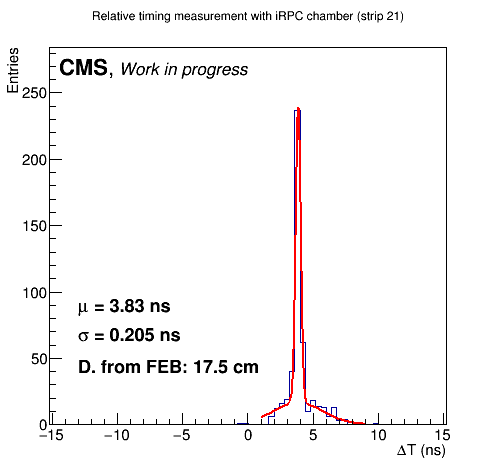
\includegraphics[width=\marginparwidth]{ELE/17p5cm.jpg}\label{17p5cm}}
	\hfill
	\subfloat[Distribution des $T^{n,21}_2-T^{n,21}_1$ lorsque le faisceau est à une distance \SI{5.5}{\centi\meter} des mezzanines.]{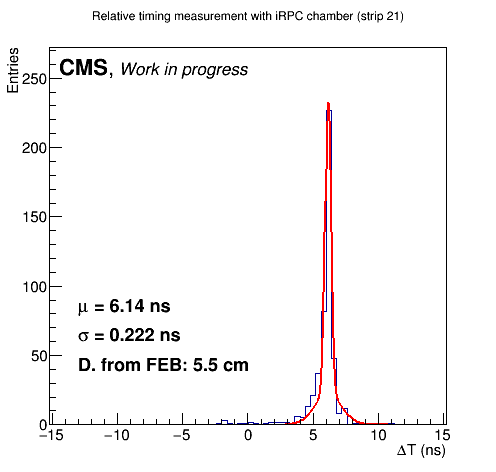
\includegraphics[width=\marginparwidth]{ELE/5p5cm.jpg}\label{5p5cm}}
	\caption{Distribution des $T^{n,21}_2-T^{n,21}_1$ pour différentes positions de la table.}
	\label{move}
\end{figure}

En ajustant ces distributions par deux gaussiennes \footnote{Les impédances n'ayant pas été bien adaptées.} et en reportant la valeur moyenne et le $\sigma$ de la Gaussienne la plus fine pour chaque distance $Y$ on obtient la figure \ref{Fit}.

\begin{figure}[!ht]
	\centering
	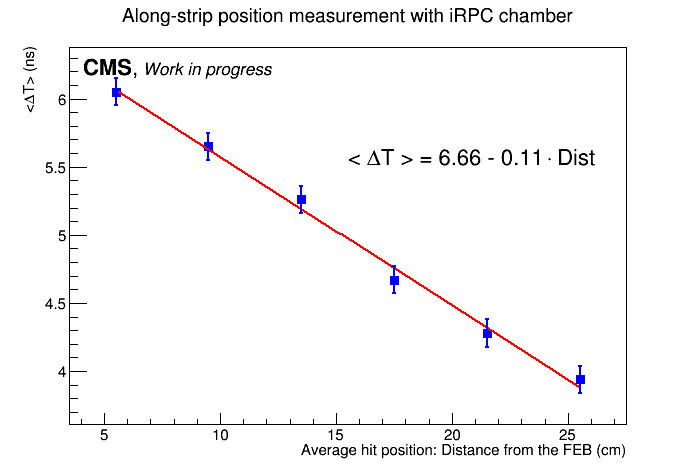
\includegraphics[width=0.7\textwidth]{ELE/MeanT_Pos.jpg}
	\caption{$<\Delta T>=<T_2-T_1>$ en fonction de la position $Y$ du détecteur.}
	\label{Fit}
\end{figure}

En ajustant la figure \ref{Fit} avec une droite et en utilisant la formule \ref{eqqq} on trouve :
\begin{equation}
v=2\frac{\dd Y}{\dd <\Delta T>}=2*\frac{1}{0.11}=\SI{18.18}{\centi\meter\per\nano\second}
\end{equation}

De plus $\sigma_{T_2-T_1}\approx\SI{200}{\pico\second}$. En utilisant la formule \ref{eqqq} il vient :
\begin{equation}
\sigma_{Y}=\sigma_{T_2-T_1}\frac{v}{2}\approx\SI{1.8}{\centi\meter}
\end{equation}

La résolution spatiale a été estimée à \SI{1.8}{\centi\meter} ce qui est très bon compte tenu des problèmes d'adaptations d'impédances et du fait que les TDC n'ont pas été correctement calibrés.

\section{Conclusion}
Le prototype de lecture des \textit{strips} des deux côtés a été testé avec deux chambres double \textit{gaps} en Bakélite de \textit{gap} \SI{1.4}{\milli\meter} (\SI{1.6}{\milli\meter}) et épaisseur d'électrodes \SI{1.4}{\milli\meter} (\SI{1.6}{\milli\meter}) qui sont les candidates privilégiées par le TDR pour l'intégration dans CMS. Malgré quelques problèmes sur la conception du PCB, nous avons pu montrer qu'il fonctionnait avec les chambres Bakélite et permettait d'obtenir une résolution spatiale de \SI{1.8}{\centi\meter} contre la longueur des \textit{strips} pour l'électronique actuelle\footnote{entre \SI{20.5}{\centi\meter} et \SI{79.72}{\centi\meter} \cite{gapss}.} tout en évitant le partitionnement en $\eta$. Ce type de lecture permet aussi de limiter le nombre de voies électroniques. En effet, en considérant la solution privilégiée par le TDR de \num{96} \textit{strips} par chambre, la solution de partitionnement en $\eta$ nécessite \num{384} voies de lecture contre deux fois moins pour le PCB à lecture des deux côtés. Tous ces avantages ont amené à privilégier cette électronique pour le TDR.